\section{Experimental Results}\label{sec:results}

\subsection{Section Organization}\label{sec:results:organization}

This section should discuss
the experimental setup and results
in your experiments.
More often than not,
it should include the following subsections.

\subsection{Experimental Setup}\label{sec:results:setup}

This subsection should discuss:
\begin{itemize}
    \item Datasets
    \item Metrics
    \item Hyperparameters
    \item Baselines
    \item Model Architectures
\end{itemize}

\subsection{Main Results}\label{sec:results:main}

This subsection should discuss:
\begin{itemize}
    \item Comparison with baselines
    \begin{itemize}
        \item Qualitative / visual results
        \item Quantitative results
    \end{itemize}
    \item Analysis and discussion
\end{itemize}

For tabular results,
follow the example below,
rendered as \Cref{tab:example}.

For plots,
include the plot ``.py'' files
in \verb|figures/| directory,
you can use \verb|figures/plot_example.py| as a template,
which is rendered as \Cref{fig:plot:matplotlib}.
Alternatively,
you may include the plot data
in a CSV file located in \verb|data/| directory,
and plot the results using TikZ + PGFPlots.
For instance,
\Cref{fig:plot:tikz} is rendered
from \verb|figures/data/plot_example.csv|.
\begin{table}[ht]
\centering
\caption{%
    An example table.
}\label{tab:example}%
\adjustbox{max width=\textwidth}{0.00\%}
    & \tpm{00.00\peta}{000.00\tera}
    & \tpm{00.00\giga}{000.00\mega} \\
Related B
    & \tpm{00.00\%}{0.00\%}
    & \tpm{\tbred{00.00\peta}}{000.00\tera}
    & \tpm{\tbred{00.00\giga}}{000.00\mega} \\
Related C
    & \tpm{00.00\%}{0.00\%}
    & \tpm{\tbred{00.00\peta}}{000.00\tera}
    & \tpm{\tbred{00.00\giga}}{000.00\giga} \\
\midrule
Method (Ours)
    & \tbpm{00.00\%}{0.00\%}
    & \tpm{\tbgreen{00.00\peta}}{000.00\peta}
    & \tpm{\tbgreen{00.00\giga}}{000.00\giga} \\
\bottomrule
\end{tabular}}
\end{table}

\begin{figure}[ht]
    \centering
    \hpad
    \begin{subfigure}{0.45\linewidth}
        \centering
        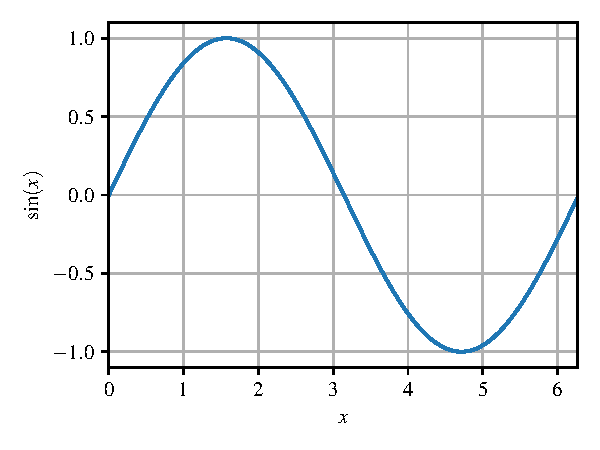
\includegraphics[width=\linewidth]{plot_example}
        \caption{%
            An example plot using Matplotlib.
        }\label{fig:plot:matplotlib}
    \end{subfigure}
    \hpad
    \begin{subfigure}{0.45\textwidth}
        \centering
        \tikzsnfn{plot_example_tikz}
        \begin{tikzpicture}
            \begin{axis}[
                cycle list/Dark2,
                width=\textwidth,
                height=0.8\textwidth,
                xlabel={\( x \)},
                ylabel={\( \sin\parens{x} \)},
                xtick={0, 1, ..., 6},
                ytick={-1, -0.5, ..., 1},
                xmin=0,
                xmax=6.28318530718,
                legend pos=north west,
                grid=both,
            ]
            \addplot +[
                line width=1.5pt, solid,
            ] table[
                x=time, y=amplitude, col sep=comma,
            ]{data/plot_example.csv};
            \end{axis}
        \end{tikzpicture}
        \caption{%
            An example plot using TikZ + PGFPlots.
        }\label{fig:plot:tikz}
    \end{subfigure}
    \hpad
    \caption{%
        Example plots.
    }\label{fig:plot}
\end{figure}

\subsection{Additional Results}\label{sec:results:additional}

This subsection should discuss
additional relevant results
that are not included
in \Cref{sec:results:main}.

\subsection{Ablation and Sensitivity Analysis}\label{sec:results:ablation}

This subsection should discuss:
\begin{itemize}
    \item Ablation analysis of model components
    \item Sensitivity analysis of hyperparameters
\end{itemize}
